\documentclass[11pt,a4paper]{letter}
\usepackage[utf8]{inputenc}
\usepackage[spanish]{babel}
\usepackage{amsmath}
\usepackage{amsfonts}
\usepackage{amssymb}
\usepackage{graphicx}
\usepackage{setspace} % Necesario para modificar el interlineado
\usepackage{comment}
\usepackage[left=2cm,right=2cm,top=2cm,bottom=2cm]{geometry}
\begin{document}
\begin{center}
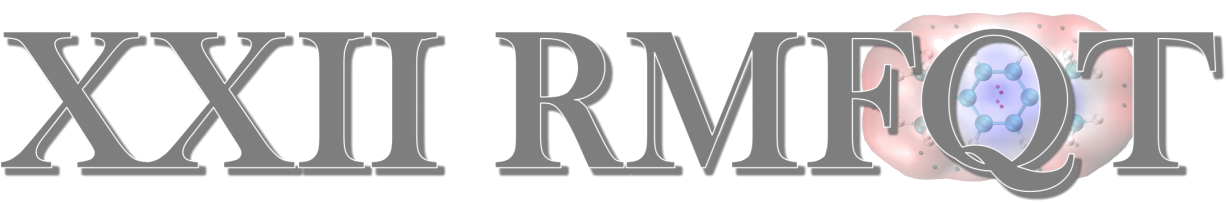
\includegraphics{rmfqt-2024}
\end{center}
\vspace{0.5cm}
\begin{center}
{\bfseries\LARGE La dimesión fractal como medida caracterizadora de la estructura de las proteínas \par}
\vspace{0.5cm}
{\itshape\Large Edgar García Juárez, J. M. Solano Altamirano, Viridiana Vargas Castro \par}
{\itshape\Large Benemérita Universidad Autónoma de Puebla (BUAP) \par}
\end{center}
\vspace{0.5cm}

\begin{comment}
La determinación de estructuras que tienen la propiedad de que su aspecto y distribución sea estadística y que no cambie a cualquiera que sea la escala a la que se analice, se presente en un gran número de sistemas complejos, como lo son las proteínas, la dimesión fractal es el índice númerico que sintetiza toda la información que contiene un sistema dinámico a analizar y puede ser utilizada para describir los rasgos de estructuras  complejas "proteícas" porque no rigen por topologías enteras y formas regulares. 

Se pretende analizar la dimesion fractal de masa y el radio de giro de varias proteínas partiendo de la definicion de multifractalidad a partir de datos experimentales.

Esperando obtener resultados que ayuden a entender si alguna region de una proteína con una mayor o menor dimensión fractal está asociada con sitios de interacción con otras proteínas o con mutaciones relacionadas, para identificar regiones específicas de una proteína que exhiba una complejidad estructural alterada en pacientes con  alguna enfermedad, para desarrollar modelos predictivos que evaluen cómo las mutaciones  afectan la estructura tridimensional y la función de alguna proteína o para saber si existen implicaciones importantes para la predicción del riesgo de desarrollar alguna enfermedad.

Escribir que se pretender encontrar una relacion entre la dimesion fractal de masa el radio de giro y la multifractalidad (explicarlo a partir del articulo del Dr. Carrillo).


Las proteínas son  estructuras complejas que exhiban propiedades estadísticas en su aspecto y distribución, independientemente de la escala de observación. En diversos sistemas biólogicos, la dimensión fractal emerge como un índice numérico que encapsula toda la información contenida en un sistema dinámico y que puede ser aplicable para describir estructuras proteicas.
\end{comment}

\onehalfspacing % Interlineado a 1.5



En diversos sistemas complejos, como las proteínas, es frecuente encontrar estructuras cuyo aspecto y distribución  sea estadístico independientemente de la escala de análisis. La dimensión fractal, como índice numérico, sintetiza la información de estos sistemas dinámicos y resulta útil para describir estructuras complejas, las cuales no tienen formas regulares ni orden aparente.


Se pretende evaluar la dimesion fractal de masa y el radio de giro de varias proteínas partiendo de la definicion de multifractalidad usando datos experimentales.

El objetivo principal es investigar como cambian los patrones de agregaciones de las proteinas y determinar si esos patrones se modifican en las proteinas, analizando si existe una diferencia entre proteínas mutadas de las sanas, lo cual podía ser relevante en enfermedades como el Alzheimer o las tubulinopatias.



\end{document}